% For submission and review of your manuscript please change the command to 
\documentclass[manuscript, screen]{acmart}
% When submitting camera ready or to TAPS, please change the command to 
% \documentclass[sigconf]{acmart}

\pagestyle{plain}

\usepackage{xspace}
\usepackage{siunitx}
\DeclareSIUnit{\fps}{fps}
\usepackage[inline]{enumitem}
\usepackage{multicol}
\usepackage{multirow}

\newcommand{\etal}{\emph{et~al.\xspace}}
\newcommand{\ie}{\emph{i.e.}, }
\newcommand{\eg}{\emph{e.g.}, }
\newcommand{\etc}{\emph{etc.\xspace}}
\newcommand{\vxv}[2]{$#1\!\times\!#2$}

\AtBeginDocument{%
  \providecommand\BibTeX{{%
    Bib\TeX}}}

% Rights management information. 
% This information is sent to you when you complete the rights form.
% \copyrightyear{2025}
% \acmYear{2025}
% \makeatletter
% \def\@ACM@copyright@check@cc{}
% \makeatother
% \setcopyright{cc}
% \setcctype{by}
% \acmConference[MM '25]{Proceedings of the 33rd ACM International Conference on Multimedia}{October 27--31, 2025}{Dublin, Ireland}
% \acmBooktitle{Proceedings of the 33rd ACM International Conference on Multimedia (MM '25), October 27--31, 2025, Dublin, Ireland}
% \acmDOI{10.1145/3746027.3758153}
% \acmISBN{979-8-4007-2035-2/2025/10}

% Submission ID.
% Use this when submitting an article to a sponsored event. You'll receive a unique submission ID from the organizers of the event, and this ID should be used as the parameter to this command.
% \acmSubmissionID{123-A56-BU3}

% If you are preparing content for an event sponsored by ACM SIGGRAPH, you must use the "author year" style of citations and references.
% \citestyle{acmauthoryear}

\begin{document}

\title[PointStream]{PointStream: A Generative AI and Pose Estimation Framework for Live Video Streaming}

\author{Emanuele Artioli}
\email{emanuele.artioli@aau.at}
\orcid{0009-0007-9921-0006}
\affiliation{
  \institution{Alpen-Adria-Universitaet}
  \city{Klagenfurt}
  \state{Kaernten}
  \country{Austria}
}
\author{Daniele Lorenzi}
\email{daniele.lorenzi@aau.at}
\orcid{0000-0003-3689-6315}
\affiliation{
  \institution{Alpen-Adria-Universitaet}
  \city{Klagenfurt}
  \state{Kaernten}
  \country{Austria}
}
\author{Farzad Tashtarian}
\email{farzad.tashtarian@aau.at}
\orcid{0000-0002-5584-6690}
\affiliation{
  \institution{Alpen-Adria-Universitaet}
  \city{Klagenfurt}
  \state{Kaernten}
  \country{Austria}
}
\author{Christian Timmerer}
\email{christian.timmerer@aau.at}
\orcid{0000-0002-0031-5243}
\affiliation{
  \institution{Alpen-Adria-Universitaet}
  \city{Klagenfurt}
  \state{Kaernten}
  \country{Austria}
}

\begin{abstract}
As video resolutions and frame rates continue to rise, a key challenge in video streaming is maintaining high quality under constrained bandwidth, especially for real-time and mobile applications. While recent work explores semantic compression and generative reconstruction to prioritize perceptually important content, many approaches still transmit large amounts of pixel data or rely on dense representations. We introduce PointStream, a real-time, object-centric streaming method that transmits only high-level information about dynamic regions—such as object positions, poses, and minimal visual descriptors—while reconstructing full frames on the client using a generative model. In our demonstration on tennis videos, we identify and extract players, rackets, and balls, and stream them efficiently to the client, while treating all other elements as part of a static background. Experiments show that PointStream achieves adequate perceptual quality of 0.2 LPIPS (or 60 VMAF) with less than 200 Kbps, whereas state-of-the-art methods for live streaming need 7 to 10 times as much bitrate to reach the same quality. We make the dataset and code available upon acceptance.
\end{abstract}

\renewcommand{\shortauthors}{Emanuele Artioli, Daniele Lorenzi, Farzad Tashtarian, \& Christian Timmerer}

% The code below is generated by the tool at http://dl.acm.org/ccs.cfm.
\begin{CCSXML}
<ccs2012>
   <concept>
       <concept_id>10010147.10010178.10010224.10010245.10010252</concept_id>
       <concept_desc>Computing methodologies~Object identification</concept_desc>
       <concept_significance>500</concept_significance>
       </concept>
   <concept>
       <concept_id>10010147.10010178</concept_id>
       <concept_desc>Computing methodologies~Artificial intelligence</concept_desc>
       <concept_significance>500</concept_significance>
       </concept>
   <concept>
       <concept_id>10002951.10003227.10003241.10010843</concept_id>
       <concept_desc>Information systems~Online analytical processing</concept_desc>
       <concept_significance>300</concept_significance>
       </concept>
   <concept>
       <concept_id>10002951.10003227.10003251.10003255</concept_id>
       <concept_desc>Information systems~Multimedia streaming</concept_desc>
       <concept_significance>500</concept_significance>
       </concept>
   <concept>
       <concept_id>10010147.10011777.10011778</concept_id>
       <concept_desc>Computing methodologies~Concurrent algorithms</concept_desc>
       <concept_significance>300</concept_significance>
       </concept>
   <concept>
       <concept_id>10010147.10010371.10010395</concept_id>
       <concept_desc>Computing methodologies~Image compression</concept_desc>
       <concept_significance>500</concept_significance>
       </concept>
 </ccs2012>
\end{CCSXML}

\ccsdesc[500]{Computing methodologies~Object identification}
\ccsdesc[500]{Computing methodologies~Artificial intelligence}
\ccsdesc[300]{Information systems~Online analytical processing}
\ccsdesc[500]{Information systems~Multimedia streaming}
\ccsdesc[300]{Computing methodologies~Concurrent algorithms}
\ccsdesc[500]{Computing methodologies~Image compression}

% Keywords. 
% The author(s) should pick words that accurately describe the work being presented. Separate the keywords with commas.
\keywords{HTTP adaptive streaming, Generative AI, End-to-end architecture, Quality of Experience}

\maketitle

\section{Introduction}
Modern video codecs consume excessive bandwidth by encoding important motion with the same priority as irrelevant visual details--an increasingly critical inefficiency, given that video streaming is ubiquitous, underpinning entertainment, education, and communication platforms, and accounting for 65\% of global Internet traffic~\cite{sandvine}. While traditional video codecs like Advanced Video Codec (AVC or H.264)~\cite{h264_overview}, High Efficiency Video Codec (HEVC or H.265)~\cite{h265_overview}, AOMedia Video~1 (AV1)~\cite{av1_overview}, \etc ~employ compression techniques such as motion estimation to significantly reduce redundancy, they still encode full frames and treat them as sequences of blocks. As a result, they lack higher-level processing, give equal priority to even imperceptible or viewer-irrelevant background changes, and fail to exploit predictable object appearance and movement. The ongoing shift to 4K (\vxv{3840}{2160}) resolution and beyond makes these inefficiencies more pronounced, wasting substantial bandwidth and storage resources.

In contrast, the human visual system processes scenes with remarkable efficiency. Rather than uniformly parsing the entire visual field, the brain focuses attention on salient objects and motion, using peripheral vision to gather low-resolution contextual cues~\cite{cajar2016spatial}. This selective attention helps manage the overwhelming volume of sensory data, allowing for rapid scene recognition and decision-making. Moreover, the brain leverages prior visual experience to anticipate familiar patterns, allowing it to infer and reconstruct missing or occluded information based on learned expectations~\cite{serences2006selective}. This combination of object-centric processing and predictive inference yields a far more efficient representation of dynamic environments than conventional video compression methods achieve.

Inspired by the efficiency of the human visual system, we propose {\em PointStream}, a novel live video streaming approach that prioritizes semantically meaningful and dynamic content over low-level pixel fidelity.
Rather than transmitting full video frames, PointStream identifies and isolates objects of interest from a static background. It tracks these objects across frames using pose estimation and encodes their motion into a lightweight representation that includes spatial positions, poses, and minimal appearance descriptors, such as edges or facial expressions in the case of people. PointStream transmits the static background once and reuses it throughout the scene, which significantly reduces the data needed for high-quality playback. It ignores non-salient motion entirely. This approach mirrors how the human visual system focuses on dynamic elements and relies on contextual understanding to fill in missing details~\cite{wu2014guidance}.
The primary contributions of this work include:
\begin{itemize}[topsep=0pt,itemsep=0pt,leftmargin=*]
\item \textbf{A novel semantic video compression scheme} that encodes salient objects with extremely low amounts of data, significantly reducing bandwidth requirements for high-quality streaming.
\item \textbf{An efficient and scalable generative model for client-side video reconstruction} that synthesizes high-fidelity images from highly compressed semantic representations.
\item \textbf{A modular end-to-end system} that integrates state-of-the-art techniques for segmentation, pose estimation, background stitching, compression, and image generation into a highly optimized semantic live video streaming pipeline.
\end{itemize}

\section{Related Work}

\subsection{Traditional video coding and streaming}
% When videos started being shared over the Internet, they were initially delivered via progressive download, where media files did not account for network conditions, or whether the viewer was interested in watching the video in its entirety~\cite{progressive}.

Leveraging the Hypertext Transfer Protocol (HTTP) as a ubiquitous and interoperable foundation, HTTP Adaptive Streaming (HAS) delivers video content over the Internet under varying network conditions. HAS enables clients to switch between video qualities based on real-time measurements of network throughput and buffer levels. Adaptive Bitrate (ABR) control, typically implemented on the client side, represents the dominant strategy for streaming at scale~\cite{sani2017abr}. Standardized HAS variants, such as Dynamic Adaptive Streaming over HTTP (DASH)~\cite{Stockhammer2011} and HTTP Live Streaming (HLS)~\cite{AppleHLS}, partition videos into small HTTP-delivered segments and encode them at multiple quality levels. Clients select the version of each upcoming segment that best matches predicted network conditions, reducing rebuffering and enhancing the overall quality of experience~\cite{QoEWhitePaper}.

As video resolutions and streaming demands continue to rise, more advanced codecs emerge to improve compression efficiency. State-of-the-art standards such as Versatile Video Coding (VVC or H.266)~\cite{vvc_overview} and AV1~\cite{av1_overview} reduce bitrates by up to 50\% compared to their predecessors, HEVC and VP9~\cite{vp9_overview}, while maintaining similar visual quality. However, these gains come at the cost of significantly increased computational complexity, particularly during encoding, which limits their practicality for real-time or low-power applications. This trade-off prompts ongoing exploration of alternative compression techniques.

\subsection{Beyond traditional codecs}

%\cite{chen2020joint,li2018efficient}

Artificial intelligence (AI) techniques offer potential advancements in video streaming. AI-driven approaches enhance traditional codec pipelines by integrating AI modules that optimize specific components, such as rate control, motion estimation, or bitrate allocation, without altering the overall codec architecture~\cite{liu2020deep, lu2019dvc}. These hybrid methods improve compression efficiency and visual quality while remaining compatible with existing standards. In contrast, end-to-end neural video codecs replace the entire traditional pipeline with deep learning models that directly learn compact representations of video content from data~\cite{lu2019dvc, chen2021nerv}. While these fully learned systems match or even exceed the compression rates of conventional codecs, they introduce even higher computational complexity, particularly during encoding, which limits their practicality for real-time or resource-constrained scenarios.

As the computational complexity of modern video codecs continues to grow---especially on the encoding side---researchers explore ways to shift some of the processing load to the client. This shift leads to the development of techniques that enhance video quality after transmission, leveraging the increasing capabilities of consumer hardware. Notable examples include client-side frame interpolation~\cite{niklaus2020softmax, xu2019quadratic} and super-resolution~\cite{ledig2017photo}, which improve perceived visual quality independently of network conditions. These approaches represent a promising direction in research, optimize natively for the rapidly increasing capabilities of modern Graphics Processing Units (GPUs), and offer a practical way to improve quality without increasing bandwidth. However, they typically operate at the pixel or texture level, applying enhancements uniformly across the frame without considering semantic content or viewer attention, limiting their potential efficiency.

\subsection{Semantic video streaming}
Research in semantic video streaming addresses this limitation by analyzing and understanding high-level scene semantics to improve encoding and transmission efficiency. Instead of treating all pixels or blocks as equally important, semantic systems prioritize key foreground objects, human figures, or action-relevant regions for detailed encoding, while allocating fewer resources to static or semantically insignificant backgrounds. Techniques for dynamic object detection and background extraction---such as Mask R-CNN~\cite{he2017mask} and other real-time segmentation models or transformer-based object trackers~\cite{meinhardt2022trackformer}---enable the isolation of moving elements, facilitating object-specific compression. Skeletal models for human representation also gain traction, especially in applications like telepresence and low-bandwidth activity capture. Methods like OpenPose~\cite{cao2017realtime} and BlazePose~\cite{bazarevsky2020blazepose} generate lightweight yet expressive skeletal representations of motion, which streaming systems transmit in place of full pixel data. The client reanimates or renders these representations, significantly reducing bandwidth without compromising perceived quality or interactivity. Integrating such semantic abstractions into streaming pipelines marks a critical shift toward perceptually optimized video delivery.

% ad targeting~\cite{yu2022semantictargeting}, surveillance systems~\cite{delvigne2022semanticsurveillance}

Despite its potential, semantic streaming remains primarily explored in adjacent domains rather than in core video compression tasks, \eg video conferencing~\cite{zhang2020semantic3d, liu2023semconf}, 360-degree video streaming~\cite{qian2018flare, xu2020seaware}, super-resolution~\cite{zhu2020semanticsr}, and autonomous driving~\cite{wang2021longshortnet}. 
Only a few studies focus on applying semantic understanding to enhance video compression directly~\cite{zhu2019semanticadaptive, hu2020taskoriented}, demonstrating that integrating segmentation results into the streaming pipeline enables more intelligent content prioritization. These approaches show promise, but they often stop at detection or segmentation and lack optimized methods for encoding and regenerating the detected objects, limiting their ability to fully exploit the bandwidth savings achievable with semantically driven compression.
\begin{figure*}
    \centering
    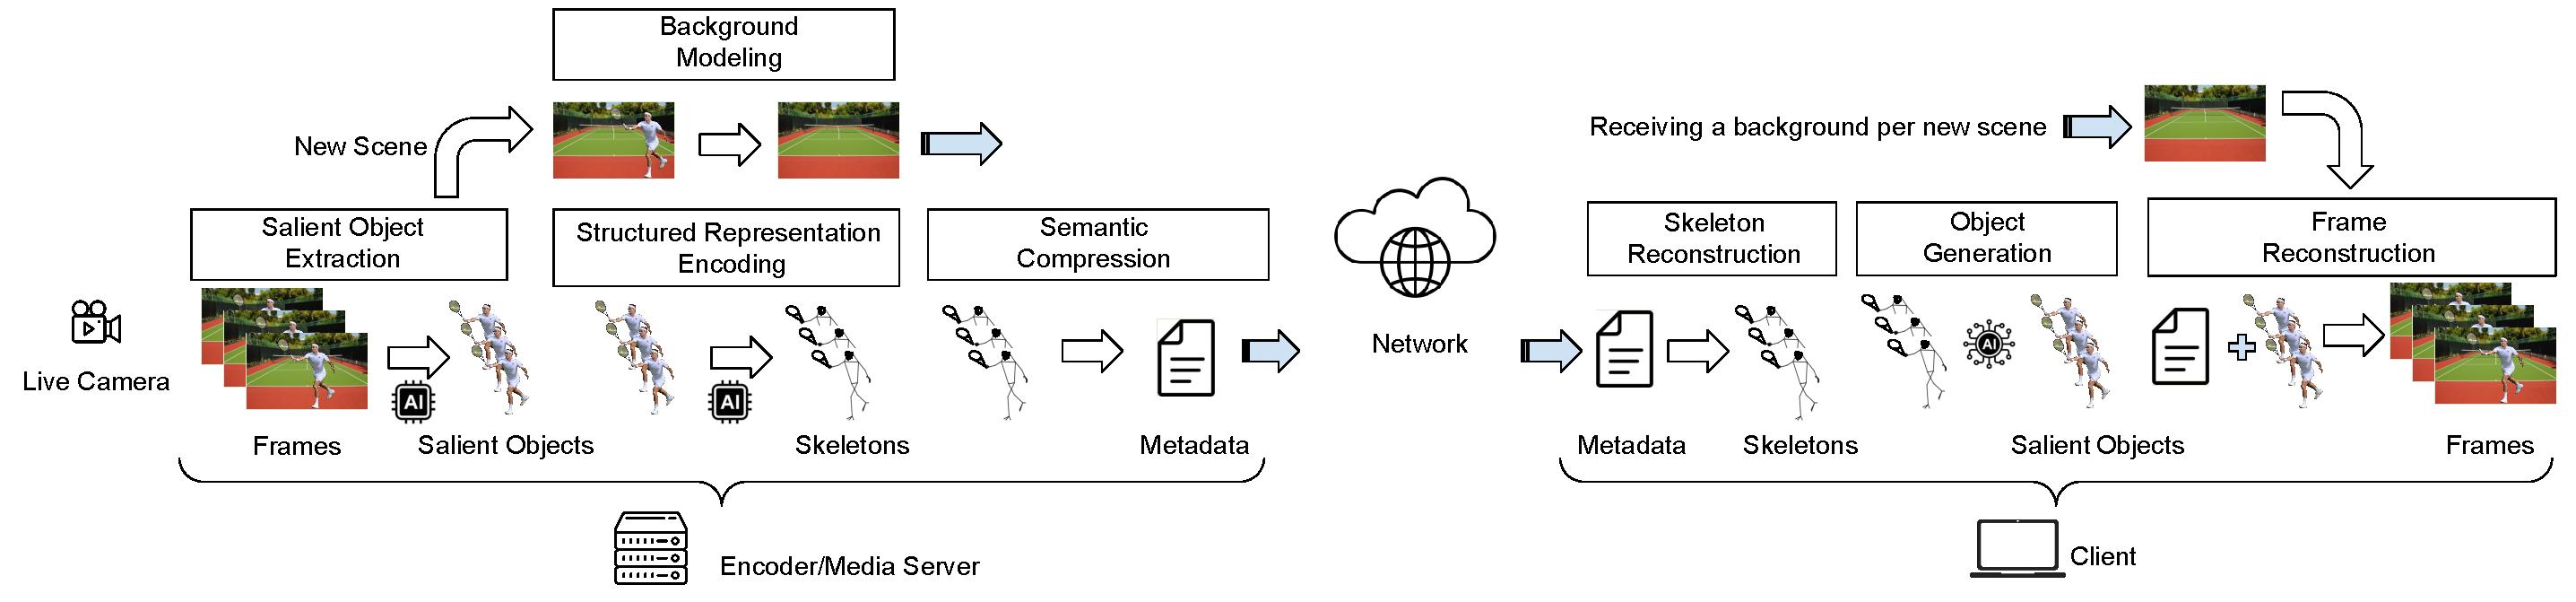
\includegraphics[width=1\linewidth]{figures/PS-overview.pdf}
    \caption{Conceptual overview of PointStream integration into the video streaming pipeline.}
    \label{fig:ps-overview}
\end{figure*}
\subsection{GenAI-based video streaming}
Advances in Generative AI (GenAI) enable impressive progress in image and video synthesis, with models that produce photorealistic scenes and animate static content~\cite{ramesh2021dalle, ho2020ddpm, isola2017pix2pix}. These models learn high-level semantic representations of objects and their motion, which makes them well-suited for applications in video streaming---particularly for reconstructing visual information from compact, abstract encodings. Despite this potential, most generative approaches remain decoupled from real-time streaming pipelines. They typically rely on private datasets and require significant computational resources to train and deploy. As a result, developers mainly use them for offline generation or post-processing, rather than integrating them directly into video compression systems.

Recent attempts explore the possibilities of integrating generative models into video streaming pipelines. For example, ELVIS~\cite{elvis} proposes a client-side inpainting framework that removes low-importance regions from transmitted frames and fills them in using a generative model at the client. This reduces the amount of background elements transmitted over the network. Although innovative, this solution still relies on traditional block-based compression and lacks deeper integration of semantic segmentation and reconstruction. As a result, it does not fully exploit object-level priors or motion-aware representations and treats each block as an isolated unit, rather than as part of a coherent object or action.

While previous work advances compression efficiency, semantic analysis, and generative reconstruction in isolation, these developments largely evolve along parallel tracks. Traditional codecs focus on low-level signal optimization, semantic systems stop at detection without optimized encoding, and generative models remain underutilized within streaming pipelines. The intersection of these trajectories reveals a clear opportunity: a unified framework that combines semantic understanding, compact representation, and generative reconstruction to enable efficient, high-quality video streaming. PointStream emerges in this space, introducing a fully object-based encoding approach that leverages scene semantics to minimize redundancy and uses generative models to reconstruct video content intelligently on the client side.

% Live video streaming has traditionally relied on two main pillars. 
% First, HTTP Adaptive Streaming (HAS) protocols use pre‐encoded representations~\cite{AVC, HEVC, AV1, VVC} to cope with network instability by dividing videos into segments and using adaptive bitrate (ABR) algorithms for quality selection~\cite{Wiegand et al. 2003, Sullivan et al. 2012}. 
% Second, content delivery networks (CDNs) and modern adaptive systems~\cite{Pensieve} have optimized client–server interactions to maintain user Quality of Experience (QoE). 
% However, despite these advances, bandwidth shortages due to network congestion and the high data demands of high-definition content persist.

% \subsection{Video compression and redundancy removal}
% Conventional video codecs exploit spatial and temporal redundancies via techniques such as motion compensation and transform coding to achieve compression. 
% While these methods have matured over decades, they often require transmitting a substantial amount of data—even for scenes with largely static backgrounds. 
% % we could talk more about how blocks of a static background with objects moving on them, need to be re-encoded every time an object occludes them, since the codec does not know what is background and what is object.
% Recently, neural video codecs~\cite{NeRV, HNeRV} have emerged as alternatives that learn compact representations of video content. 
% Although promising, such approaches tend to shift the computational burden to the client and are not yet optimized for the real‐time constraints of live streaming.

% \subsection{Neural Video Restoration and Fidelity Reconstruction}
% Parallel to advancements in compression, deep learning–based video restoration techniques have been explored to enhance perceptual quality from low-bitrate or compressed streams. 
% Methods for frame interpolation, super-resolution, and inpainting~\cite{ELVIS} use convolutional neural networks and generative adversarial networks to recover high-quality visual details. 
% Yet, these approaches generally target the entire frame without explicitly exploiting the fact that many live streams exhibit predominantly static backgrounds. 
% In contrast, our method specifically targets scenarios where background elements remain largely unchanged while objects or people move—allowing the client to reconstruct high-fidelity static content using generative models, thereby reducing client load and transmitted data volume.

% \subsection{Content-aware adaptation in live streaming}
% A growing body of work has recognized that not all video segments are equally sensitive to quality degradation. 
% For instance, SENSEI~\cite{Zhang et al., NSDI '21} demonstrates that user sensitivity to quality changes varies dynamically with content—for example, rebuffering during a crucial moment in a live event is more detrimental than during routine play. 
% % this is why we base our segments into scenes instead of seconds.
% Similarly, recent systems like GRACE~\cite{Cheng et al., NSDI '24} leverage neural codecs to improve resilience against packet loss by reconstructing missing content on the fly. 
% These studies underscore the potential of incorporating semantic or content-aware insights into streaming systems. 
% Our work builds on this idea by concentrating on fidelity reconstruction of static scenes; by transmitting only essential motion information, we can devote computational resources at the client side (on modern GPUs) to reconstruct the crucial elements of a video with high visual fidelity.

%\newpage

\section{Problem Description and Motivation}

% \begin{figure}
%     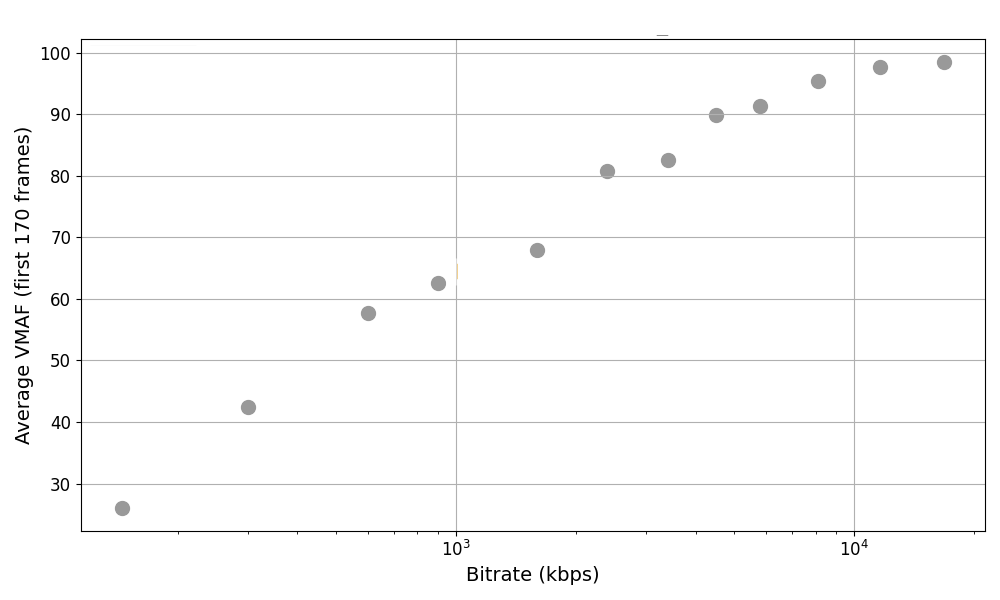
\includegraphics[width=\columnwidth]{figures/hls-vmaf.png}
%     \caption{Which Figure should we add here ???}
%     \label{fig:avg_vmaf_vs_bitrate}
% \end{figure}

To evaluate whether our approach brings meaningful improvements in video quality and bandwidth utilization efficiency, we first establish a baseline by measuring the performance of current state-of-the-art codecs under constrained bandwidth conditions, and apply it to a tennis match segment at 4K resolution, framerate of \SI{50}{\fps} and \SI{8}{\second} of duration.
As our reference codec, we select HEVC due to its widespread adoption and high compression efficiency. 
We encode the target video\footnote{\url{https://www.youtube.com/watch?v=7QoKrvOvIGw&t=88s}, last access: 2025-04-11.} at each bitrate among the representations in the Apple HLS bitrate ladder~\cite{AppleHLS} for adaptive streaming results in a quality between \SI{27}{VMAF} at 360p (\vxv{640}{360}) resolution and 145\,Kbps bitrate, up to basically flawless reconstruction at 4K and 11\,Mbps. 
% As shown in Figure~\ref{fig:avg_vmaf_vs_bitrate}, 
% Encoding the target video under these conditions 

Given the structured nature of tennis video segments, we explore a content-aware alternative that exploits the inherent redundancy in the scene. 
A typical broadcast consists of 
\begin{enumerate*}[label=\textit{(\roman*)}] 
\item a static background (court, audience, advertising boards), and 
\item a few dynamic elements (players, rackets, ball)
\end{enumerate*}.
Instead of encoding all pixels in every frame, we propose a simple yet effective optimization:
\begin{itemize}[topsep=0pt,itemsep=0pt,leftmargin=*]
    \item Extract and store only the moving objects (players, rackets, and ball) as separate video streams.
    \item Compress and store the background as a single static image.
\end{itemize}
This approach ignores irrelevant motion (\eg minor spectator movements, referees), while significantly reducing bitrate consumption when compared with the 4K representation of the benchmark.
Indeed, from the \SI{11}{MB} of the benchmark video, we move to a \SI{2.4}{MB} 4K background, plus two \SI{950}{KB} and \SI{1.2}{MB} video files respectively for players, a saving of \SI{6.45}{MB}, or about \qty{60}{\percent}.
% We are here assuming that the drop in VMAF caused by encoding a static background, does not represent a real drop in perceived video quality. Whether this assumtion is correct, is deemed outside of the scope of the present motivating example.

Despite the impressive gains, this method still requires encoding full pixel-based representations of moving objects, leaving room for further improvements.
We observe that players are humans whose motion can be efficiently represented using structured pose information. 
Leveraging this insight, we take an additional step:
\begin{itemize}[topsep=0pt,itemsep=0pt,leftmargin=*]
\item Instead of encoding pixel-level video streams for each player, we extract their 2D pose trajectories using a state-of-the-art pose estimator (\eg YOLO~\cite{redmon2016yolo}) and represent their motion over time as a sequence of keypoints.
\item We employ a lightweight generative model (\eg  Conditional Generative
Adversarial Network (cGAN)~\cite{isola2017pix2pix}) to reconstructs plausible visual representations of the players conditioned on these pose sequences.
\end{itemize}
This transformation yields another substantial reduction in data size, from the previous \SI{950}{KB} and \SI{1.2}{MB} to \SI{230}{KB} and \SI{294}{MB}, or about \qty{75}{\percent} smaller than the object-video approach, and a total reduction from \SI{4.55}{MB} to \SI{2.92}{MB}, another \qty{36}{\percent} size drop.
% Once more, we forgo to calculate VMAF for these experiments, and instead assume that the client side generative model would be able to replicate players without noticeable artifacts.

We note that these results assume that the perceptual impact of certain approximations is negligible. 
In particular, encoding the background as a static image may reduce objective quality metrics such as VMAF, but we posit that this does not reflect a meaningful drop in perceived quality, given the minimal motion and low saliency of those background elements.
Similarly, in the pose-based reconstruction case, we assume that the generative model produces visually plausible outputs sufficient to maintain perceived fidelity. 
While these assumptions simplify the evaluation, they are reasonable within the controlled scope of this illustrative example.

Although not intended as a rigorous or statistically comprehensive evaluation, this stepwise transformation, from full-frame encoding, to object-background separation, to structured motion-based representation, highlights the potential of a content-aware, human-centric approach. 
These insights directly inform the design of our proposed system, \emph{PointStream}, which generalizes this paradigm into a scalable and modular semantic live streaming pipeline.

\section{System Design}

Unlike traditional designs that encode and transmit dense pixel grids, PointStream leverages object-centric scene understanding to transmit only the perceptually significant elements of each frame.
It identifies salient elements in a scene and encodes them as compact representations that preserve only essential motion and appearance information. 
Static or low-importance regions are handled separately, using efficient background modeling. 
The structured nature of these representations enables significant compression gains through semantic-aware encoding. 
At the client side, full video frames are reconstructed via learned models that synthesize visuals from the compressed descriptions, reassembling a coherent and high-quality scene. 
Figure~\ref{fig:ps-overview} presents a conceptual overview of the end-to-end PointStream architecture, from the encoder/media server to the client, highlighting its key components.

\subsection{Server-side PointStream}
The server-side pipeline of PointStream is designed to convert raw video frames into a highly structured, bandwidth-efficient representation of dynamic content. It consists of four primary components: salient object extraction, structured representation encoding, background modeling, and semantic compression (see Figure~\ref{fig:ps-overview}).

\subsubsection*{Salient object detection}
This process begins with the identification and isolation of salient, temporally evolving elements within the scene. 
These objects are extracted based on their visual distinctiveness, motion patterns, and contextual relevance, using a combination of segmentation, tracking, and feature extraction techniques. 
The goal is to reduce the visual scene to a minimal set of meaningful entities that drive the viewer’s attention and overall scene understanding, and consider any other part of the scene as background.

\subsubsection*{Structured representation encoding}
For each extracted object, the system generates a compact representation that captures its essential spatial configuration and temporal dynamics. 
These representations, obtained with state-of-the-art (SOTA) keypoint extraction models, are chosen to be compact in size yet expressive enough to enable plausible reconstruction downstream. 
By focusing on structured features such as movement trajectories and overlaps, the system avoids the inefficiency of pixel-level redundancy inherent in traditional codecs.

\subsubsection*{Background modeling}
% In parallel, the server constructs a stable and artifact-free background model by retaining static or low-motion regions across the video, while removing the portions corresponding to the salient objects, and substituting them with portions of the background at a different time, where the object has moved away and the background area that was occluded is here visible.
% This stitched background is treated as a slowly varying or static layer, which can be transmitted once or updated infrequently.
% By separating background and foreground content, PointStream avoids repeatedly encoding visual information that does not contribute to perceptual change.
A core challenge in live streaming is handling both periods of stable camera work (e.g., a tennis rally) and abrupt scene changes (e.g., cuts to replays or spectator close-ups). PointStream addresses this with a hybrid approach that begins by segmenting the video stream in real-time. The system analyzes frame-to-frame similarity to detect camera cuts and significant global motion.

For stable scenes, the server constructs a background model by retaining static or low-motion regions across the video, while removing the portions corresponding to the salient objects, and substituting them with portions of the background at a different time, where the object has moved away and the background area that was occluded is here visible.
This stitched background is treated as a slowly varying or static layer, which can be transmitted once or updated infrequently.
By separating background and foreground content, PointStream avoids repeatedly encoding visual information that does not contribute to perceptual change.

Conversely, when the camera shifts quickly, the current stable scene is terminated. The subsequent segment is encoded using a traditional video codec. This ensures robust handling of any video content. The system continuously monitors for a return to a stable camera view to begin handling a new stable scene. This hybrid design allows PointStream to apply its powerful semantic compression where it is most effective, while gracefully handling the full range of dynamic content found in a typical live broadcast.

\subsubsection*{Semantic compression}
The final step on the server involves encoding the object representations into a highly compressed transmission format. Thanks to the structured nature of the data, this format is highly optimized.
The encoding includes object-specific information such as spatial location and salient features, and results in a compact and intelligent scene abstraction that prepares the client for high-quality generative reconstruction with minimal data. It is worth noting that, in PointStream, the data of salient objects extracted from each frame is encoded and delivered to the client at intervals aligned with the target latency requirements of live video streaming applications.

% The server-side processing is responsible for extracting dynamic objects from input frames. This is achieved through a combination of image segmentation, object tracking, and pose estimation techniques. These methods allow the system to isolate relevant objects, determine their shape, and track their evolution over time. The extracted representations of the objects contain minimal data to enable accurate reconstruction on the client side. Additionally, the server constructs a clean representation of the scene background by aggregating static elements across multiple frames. This background reconstruction enables the client to focus on rendering dynamic content without redundant transmission of unchanging or non-salient visual elements.
% Once the objects have been extracted, their representations are encoded into a compact format for transmission. The encoding is designed to balance efficiency and fidelity, ensuring that only essential information is relayed while preserving the integrity of motion and appearance. The system employs a structured format that includes object bounding regions, key spatial features, and temporal consistency constraints.

\subsection{Client-side PointStream}
The client-side component of PointStream is responsible for transforming the compact, structured scene description into a complete visual reconstruction. To achieve this, PointStream introduces three key modules on the client side: skeleton reconstruction, object generation, and frame reconstruction (see Figure~\ref{fig:ps-overview}).
\subsubsection*{Skeleton reconstruction}
Upon receiving the semantic representations of dynamic objects, the client decodes them with extreme efficiency. Having obtained the uncompressed keypoint values of each salient object, it leverages a generative synthesis model to reconstruct visually plausible frames. 
\subsubsection*{Object generation}
Rather than decompressing pixel-by-pixel information, the client interprets the abstracted data, such as spatial configuration, motion trajectories, and salient object attributes, to infer the appearance and behavior of each scene element.
Crucially, this process enables the client to regenerate rich visual content from minimal inputs, guided by learned priors and contextual expectations.
The generative model fills in fine-grained visual details, ensuring temporal coherence and seamless integration between dynamic objects and background elements.
This mirrors how human vision fills in visual gaps based on prior experience and motion continuity.
\subsubsection*{Frame reconstruction}
In the final stage, the client assembles each frame by attaching the generated salient objects—such as the player, racket, and ball—to the most recently received background frame. This process uses the precise spatial coordinates of each salient object, as provided by the server, to ensure accurate placement and alignment. Once all frames in the segment have been reconstructed, they are passed to the video player for real-time rendering and playback.

By offloading reconstruction tasks to the client, PointStream reduces the server’s computational burden and minimizes transmission bandwidth. 
The client’s role is no longer passive; instead, it actively participates in rendering the final experience. 
This division of responsibilities allows PointStream to scale flexibly across devices and scene complexities by sending appropriate models to each client based on their computational capabilities, supporting high-fidelity playback under tight bandwidth constraints.

% On the client side, the received representations are processed to synthesize the missing visual information and reconstruct a complete scene. A generative model is utilized to infer details and blend dynamic objects seamlessly into the scene. This allows the client to render a visually coherent sequence while significantly reducing bandwidth.
% The division of labor between server and client ensures that the system can scale across different scene types while maintaining high fidelity and efficiency.

\section{Performance Evaluation}

\subsection{PointStream implementation}
To validate our approach, we applied the system to the analysis of tennis matches.
Tennis serves as an ideal test case due to its structured environment, where the primary dynamic elements, \ie players, rackets, and balls, move against a largely static background. 
This setup allows for efficient segmentation and reconstruction of relevant objects while minimizing interference from extraneous scene elements.
For this work, we collected and curated a dataset of tennis videos from top-level tournaments, which serves as the foundation for our implementation and will be detailed later in this section.
The processing pipeline, implemented in Python, handles video processing, object and keypoint extraction, background stitching, optional object segmentation for model training, and the client-side components.
The entire project is packaged into two Docker~\cite{merkel2014docker} containers—namely, server and client—and deployed on a local Ubuntu 20.04 LTS server equipped with an Intel Xeon Gold 5218 CPU (64 cores, 2.30 GHz) and an NVIDIA Quadro RTX 8000 GPU with 48 GB of memory.

% \subsubsection*{Video processing and object detection}
% The system processes input videos by extracting frames with FFmpeg~\cite{ffmpeg} and applying YOLO~\cite{redmon2016yolo}, an object detection model, to identify every object within each scene. 
% To capture fast-moving elements prone to motion blur, YOLO is configured with a confidence threshold of \num{0.25} and an Intersect over Union (IoU) threshold of \num{0.1}, values lower than typical settings. 
% While this improves detection recall, it also increases the number of recognized elements, leading to higher computational demands. 
% Despite YOLO’s efficiency, handling an excessive number of detections presents a challenge, requiring an optimized selection mechanism.

\subsubsection{Scene Analysis and Object Detection}
Our server-side implementation begins by processing the input video stream to segment it into distinct scenes. Using FFmpeg~\cite{ffmpeg}, frames are extracted and analyzed for camera cuts via a high-throughput frame difference algorithm. A sequence of frames between two cuts that maintains a stable camera perspective is classified as a stable scene, making it eligible for our semantic compression pipeline. All other segments, such as replays, close-ups, or rapid camera pans, are routed directly to a traditional video encoder, ensuring robust handling of all content.

For frames within an identified stable scene we proceed with salient object detection using YOLO~\cite{redmon2016yolo}. To effectively capture fast-moving elements like a tennis ball or racket, which are often subject to motion blur, YOLO is configured with deliberately sensitive parameters: a confidence threshold of \num{0.25} and an Intersect over Union (IoU) threshold of \num{0.1}. While lowering these thresholds from their typical settings improves detection recall for crucial small or fast objects, it also increases the overall number of recognized elements. Despite YOLO’s efficiency, handling an excessive number of detections presents a challenge, requiring an optimized selection mechanism.

\subsubsection*{Object association}
To streamline processing, only objects of interest, \ie players, rackets, and balls, are retained, while all other detections are labeled as part of the background. 
Since many people appear in the scene but do not participate in gameplay, further refinement is necessary to distinguish between players and bystanders. 
This is achieved by associating rackets with players based on the spatial overlap of their bounding boxes.
Rackets, due to their rapid motion, are often detected inconsistently across frames. 
To address this, once a racket is linked to a player, the system continuously tracks that player, dynamically adjusting their bounding box in subsequent frames to ensure their racket remains within the detection region, even if temporarily unrecognized.

\subsubsection*{Data storage}
Once objects have been categorized and associated, they are stored systematically. 
Each detected instance is cropped and saved into object-specific directories, while bounding box coordinates are recorded for later use and transmission. 
To maintain focus on salient content, only individuals consistently identified as players across the video are retained.
Other people, who may have appeared briefly or were never linked to gameplay elements, are treated as bystanders and added to the background.
This pruning process reduces noise and ensures that only meaningful dynamic elements are preserved for downstream synthesis.

\subsubsection*{Keypoint extraction}
\begin{figure*}
    \centering
    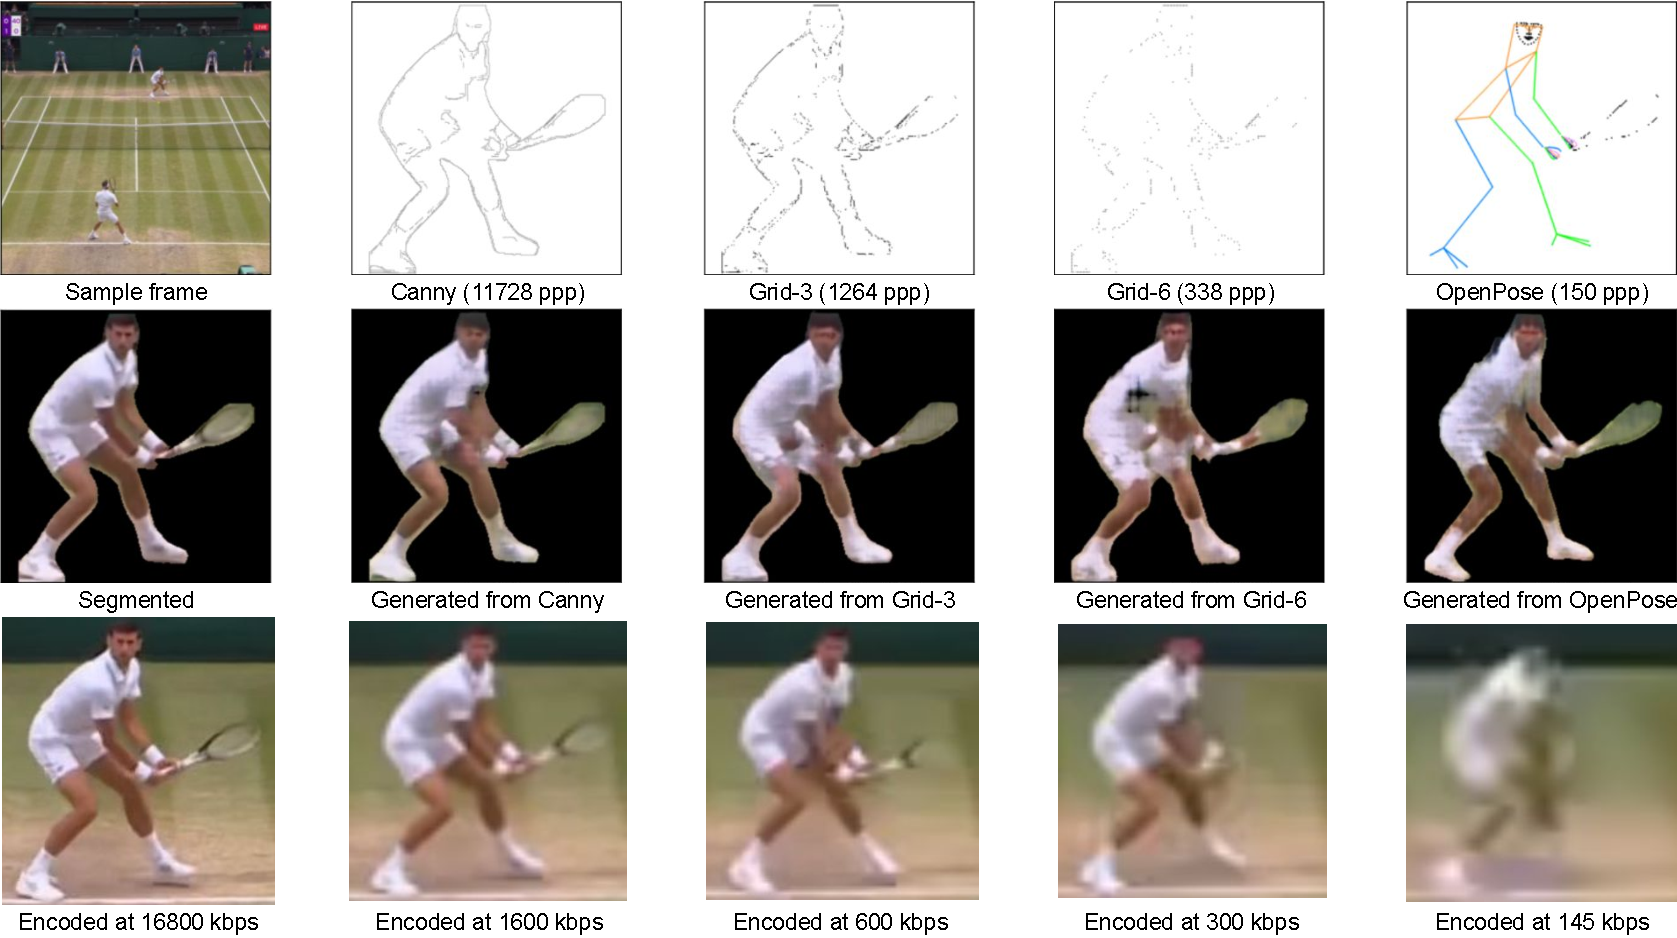
\includegraphics[width=1\linewidth]{figures/players.pdf}
    \caption{Qualitative comparison between the player image generated from different keypoint methods (middle row), and the player cropped from videos encoded at similar bitrates. It is worth noting that the input map for OpenPose is obtained by merging the OpenPose skeleton keypoints with the Canny keypoints of the racket.}
    \label{fig:qualitative-result}
\end{figure*}
After detecting and filtering objects, the system advances to a keypoint extraction stage. 
This phase focuses on converting each object of interest, \ie players, rackets, and the ball, into a structured set of spatial coordinates that compactly represent their visual and motion characteristics. 
Since bounding boxes have already been computed in the detection phase, keypoint extraction can be performed in parallel, substantially improving processing speed.
For players, we rely on a set of pose estimation strategies designed to capture relevant anatomical or structural features. 
To evaluate the trade-offs between precision and computational complexity, we employ the following approaches. The first approach applies the Canny filter~\cite{mcilhagga2011canny} to detect edges in the input image, capturing both the player and the racket. The second and third approaches build on this by using grid-based sampling with different cell sizes—3×3 (Grid-3) and 6×6 (Grid-6)—to sample a subset of points from the detected edges.
The fourth approach leverages OpenPose~\cite{cao2017realtime}, which provides \num{133} anatomical landmarks across the face, torso, and limbs. When a racket is present in the image, we additionally apply the Canny filter to the racket region and select up to 17 representative points, resulting in a total of 150 keypoints.

This final method strikes a good balance between expressiveness and efficiency, making it well-suited for fast-paced activities such as tennis. In scenarios where players face away from the camera and facial landmarks cannot be reliably detected, we use a fallback mechanism that applies grid-based sampling to the back of the head, ensuring a consistent number of 150 keypoints.

Figure~\ref{fig:qualitative-result} gives a detailed breakdown of each scheme, both in terms of their encodings, and the tennis player images that can be generated based on them.
These alternatives offer different balances between spatial resolution, robustness to occlusion, and computational cost and can be substituted depending on the desired fidelity of reconstruction or bitrate constraints.
% For rackets, which tend to be detected intermittently due to their rapid motion and slim profile, we apply a separate edge- and grid-based extraction method that yields \num{17} keypoints summarizing the object’s shape and orientation.
Finally, for the ball, which frequently appears blurred due to high speed, we extract its center point and estimate motion blur characteristics, namely elongation and direction, by analyzing its displacement across frames. This allows the client to reconstruct a plausible appearance and motion trajectory despite the lack of fine-grained visual features.

\subsubsection*{Background reconstruction}
Once all frames and objects have been processed, the system reconstructs the background by aggregating multiple frames that had their dynamic objects obscured. 
In other words, regions of the background that were occluded by the moving objects, are filled with information from other frames where these objects are in a different location.
The extracted segmentation masks and keypoints are stored alongside their corresponding bounding box data.

\subsubsection*{Data export}
Finally, the extracted coordinate data -- comprising object bounding boxes and keypoints -- is saved to a CSV file and then encoded for transmission using one of two strategies, depending on the keypoint format employed.
For fixed-size, deterministic representations such as OpenPose skeletons, we convert the coordinates into a compact raw bitstream. 
Each coordinate is encoded as a 12-bit unsigned integer, sufficient to represent pixel positions within a 4K-resolution frame (up to 3840 pixels). 
Crucially, because the number and ordering of keypoints are fixed and known in advance, each segment of the bitstream corresponds to a specific coordinate of a specific object in a deterministic way. 
For example, the first 12\,bits always encode the X-coordinate of the first keypoint of Player 1, the next 12\,bits the corresponding Y-coordinate, and so on. 
This layout removes the need for additional metadata, enabling both tight compression and extremely fast parsing on the client side. 
If an object is not detected in a particular frame, a sentinel control value (4000, greater than 3840 and thus outside the possible coordinate range) is inserted in place of the missing coordinates. 
This allows the client to gracefully handle missed detections while maintaining alignment with the expected bitstream format. 
For alternative formats such as coarse or fine spatial grids, where the number or ordering of keypoints may vary slightly between frames or objects, we apply zlib~\cite{gailly2004zlib} compression to the full coordinate CSV data. In the case of Canny-derived keypoints, we first compress the binary edge images—where each pixel is represented using only 1 bit (black or white) instead of the typical 8-bit grayscale—resulting in significant space savings. 
It is worth noting that the compressed data is delivered to the client at intervals, aligned with the target latency requirements of live video streaming applications.

% While this approach yields slightly larger files and slower decompression, it supports more flexible object representations and remains efficient in practice due to the repetitive nature of spatial patterns across frames.
% This dual strategy allows PointStream to flexibly balance compression efficiency and representational richness, depending on the desired fidelity or object class.

% Such an optimized encoding results in players and ball having a predictable impact on the video's bitrate of 40kbps for a 4K video stream.

\subsubsection*{Client-side processing and reconstruction}
Upon receiving the compressed bitstream, the client decodes the data based on the approach employed at the server side. If the server uses OpenPose and sends up to 150 keypoints, the client reconstructs the skeleton of the player and the racket, if present. In contrast, for the Canny or grid-based approach, the client generates a binary image (see the first row of Figure~\ref{fig:qualitative-result}). Using either the skeleton or the binary image, the client then employs a generative AI network to reconstruct the salient objects accordingly.

% by leveraging the fixed structure of the encoding format. 
% Since the order and number of keypoints are known a priori, each coordinate can be efficiently extracted without additional metadata. 
% These keypoints are then used to reconstruct a 2D pose skeleton for each object.

To visually recreate the players, we employ a Conditional Generative Adversarial Network (cGAN) inspired by the Pix2Pix~\cite{isola2017pix2pix} architecture, implemented using the TensorFlow~\cite{tensorflow2015} framework.
This model is trained on paired image data: each training example consists of a synthetic pose image rendered from the extracted keypoints, and the corresponding ground truth frame showing the actual player. 
Given a pose skeleton as input, the model generates a plausible photorealistic rendering of the player, which is then composited into the static background to complete the reconstructed frame.

% Upon receiving the compressed data, the client unpacks it following a reverse process than the server.
% To recreate the players at the client-side, we designed and trained a Conditional Generative Adversarial Network (cGAN) model, inspired by the Pix2Pix~\cite{isola2017pix2pix} architecture, and implemented it using the PyTorch~\cite{ketkar2021pytorch} framework.
% The model operates on paired image data where each sample comprises an image representing the player's skeleton (or estimated pose), generated based on the keypoints sent over by the server, and the ground truth image of the player.

%The generator uses a U-Net~\cite{} architecture with eight downsampling and seven upsampling blocks. Downsampling employs convolutions, batch normalization, and LeakyReLU, while upsampling uses transposed convolutions, batch normalization, and ReLU. Early upsampling layers include dropout to prevent overfitting. Skip connections help retain fine details.

%The discriminator uses a PatchGAN~\cite{} architecture, classifying image patches instead of the whole image. It processes the concatenation of the generated (or real) image and its condition image. The network has seven downsampling blocks, zero padding, and two convolutional layers, outputting a feature map that assesses patch realism.

% Both the generator and discriminator use binary cross-entropy as loss function, driving the generator to create realistic images and the discriminator to differentiate real from generated ones. 
% Additionally, the generator incorporates L1 loss to penalize deviations from the target image, ensuring structural fidelity and reducing blurriness. 
% Furthermore, the network was trained using the Adam solver~\cite{kingma2014adam} with learning rates of $2e^{-4}$ and $1e^{-4}$ for the generator and discriminator, respectively, and a momentum term $\beta_1 = 0.5$. 
% We trained the model for 40,000 steps with a batch size of 1.

The training process for the generative model combines multiple objectives to ensure both realism and structural accuracy. 
Binary cross-entropy loss is used for both the generator and discriminator, encouraging the generator to produce realistic images and the discriminator to effectively distinguish between real and synthesized samples. 
To further enforce spatial consistency and reduce blurriness, the generator is also trained with an L1 loss, which penalizes pixel-wise differences from the ground truth images.
Training is performed using the Adam optimizer~\cite{kingma2014adam}, with learning rates of $2 \times 10^{-4}$ for the generator and $1 \times 10^{-4}$ for the discriminator, and a momentum parameter of $\beta_1 = 0.5$. 
The network is trained for \num{20000} steps with a batch size of \num{1}, and its loss function progression is shown in Figure~\ref{fig:model-loss}.

\begin{figure*}
    \centering
    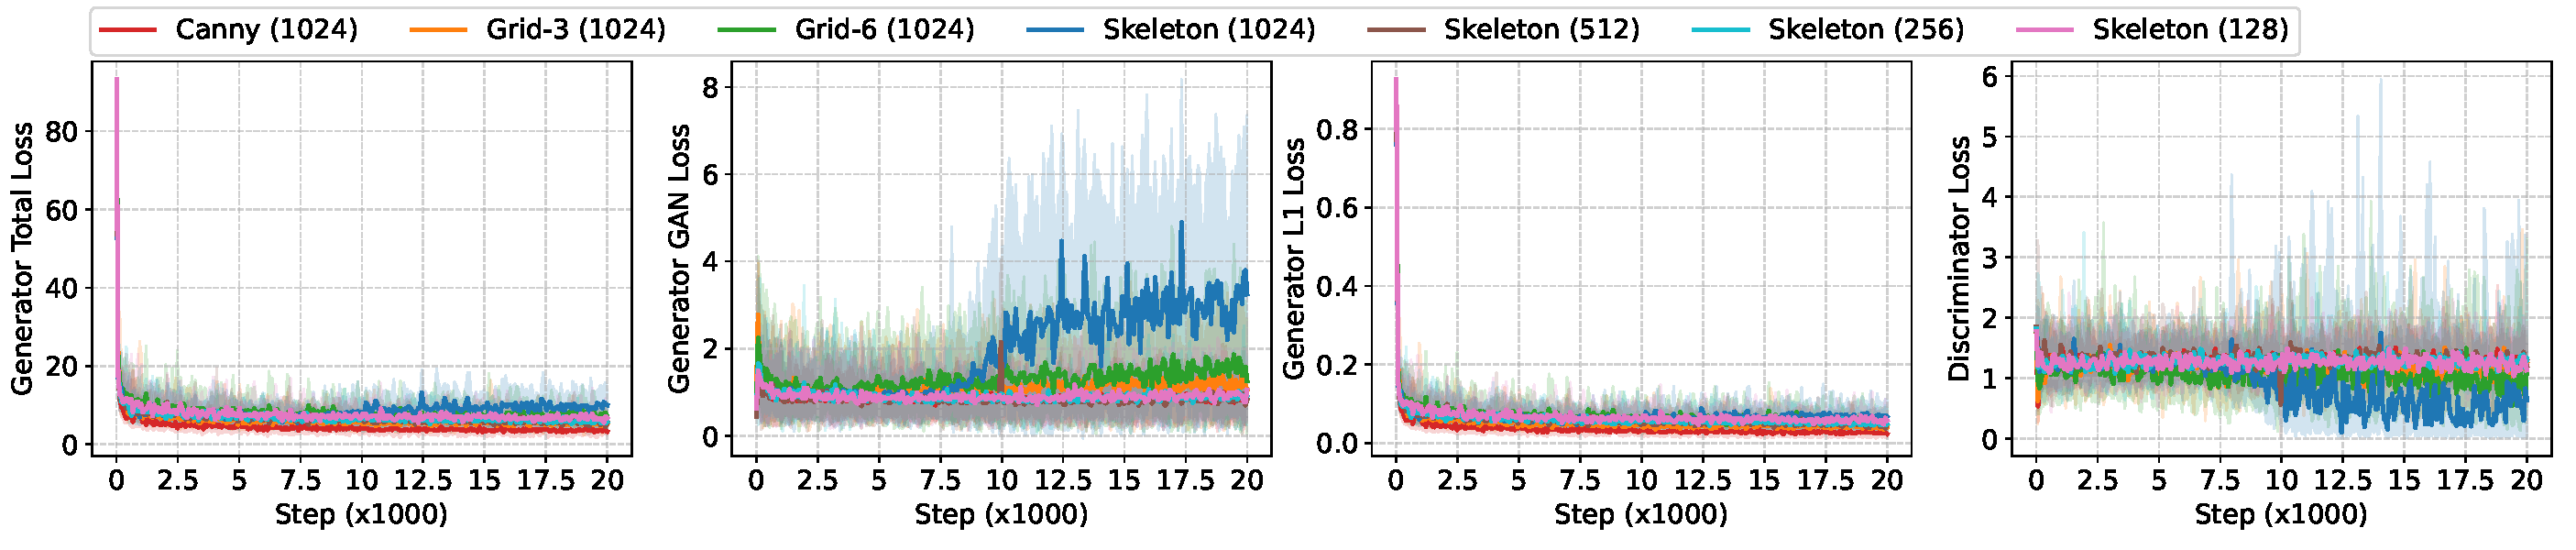
\includegraphics[width=1\linewidth]{figures/cgan_performance.pdf}
    \caption{Network loss progression over \num{20000} epochs for generator and discriminator across the adopted methods and input/output image resolutions (1024 $\rightarrow$ 1024$\times$1024, 512 $\rightarrow$ 512$\times$512, 256 $\rightarrow$ 256$\times$256, 128 $\rightarrow$ 128$\times$128).}
    \label{fig:model-loss}
\end{figure*}


% The L1 loss is weighted with the coefficient $\lambda = 100$ to control the trade-off between image realism and pixel-level accuracy. 
% The discriminator loss is also based on binary cross-entropy and measures its ability to distinguish real from generated images.

%During inference, the generator model—restored from the latest checkpoint—was applied to the test set images. The predictions were scaled to $[0, 255]$ and saved in PNG format. A visualization module displayed the input, ground truth, and generated images side by side to facilitate qualitative evaluation.

% Number of training and testing images (pairs)
%For each scene described in Section~\ref{subsubsec:content}, the training images form a set of X elements, while training is limited to Y elements. % cropped, mini-batches, augmented, etc.
% Models info, (hyper)parameters, etc.

% The model is player-specific, meaning the same network is trained multiple times, each time using only images of a specific player. This ensures that each trained model generates images only of the corresponding player.

The current implementation trains a separate generative model for each individual player, meaning that the network is re-trained multiple times using only the image data corresponding to a specific player. 
While this ensures that each model can accurately reconstruct the appearance and motion style of its associated player, it introduces a scalability limitation: a new model must be trained for every new player.
We recognize that this approach is not optimal, especially given the visual and motion similarities shared among tennis players. 
A more scalable solution would involve training a single, generalized model capable of synthesizing any player from a shared representation. 
Developing such a model remains an exciting direction for future work. 
For the scope of this paper, however, we focus on demonstrating the feasibility and effectiveness of the overall system pipeline.
% Other generalization approaches with input conditioning on the specific players have not been covered in this work

% We apply PyTorch framework to implement the proposed network on the desktop computer with 4.2GHz Intel i77700K CPU, 64G RAM, and NVIDIA TITAN Xp GPU (12G memory).

\subsection{Experimental settings}

This section provides a comprehensive overview of the experimental settings employed in the performance evaluation of PointStream. 
To improve clarity, we categorize them according to their respective domains, including \textit{content}, \textit{encoding}, \textit{training and testing}, and \textit{evaluation metrics}.

\subsubsection*{Content}\label{subsubsec:content}

In our experiments, we used a dataset comprising more than \num{10000} frames grouped in \num{20} scenes with duration ranging from \qtyrange{8}{19}{\second} extracted from two tennis matches at \qty{50}{\fps} and 4K (\vxv{3840}{2160}) resolution~\cite{tennistv}.
These scenes share key characteristics, including:
\begin{enumerate*}[label=\textit{(\roman*)}]
\item a static background with predominantly stationary objects and spectators,
\item two tennis players actively moving within their respective halves of the court, and
\item a yellow ball traversing back and forth across the court.
\end{enumerate*}
% Are the two players the same in all scenes?

\subsubsection*{Encoding}
Our goal is to evaluate PointStream's performance compared to the state-of-the-art video codec HEVC in terms of compression efficiency, \ie the trade-off between video quality and file size, and computation cost. 
Therefore, we adopted FFmpeg~\cite{ffmpeg} to encode each scene using the \textit{ultrafast} preset of the HEVC library \textit{libx265}. 
We generated a total of \num{12} representations with segments of length \qty{1}{\second}, \qty{2}{\second} and \qty{4}{\second}, according to the Apple HLS bitrate ladder~\cite{AppleHLS}. % In the comparisons reported in Section~\ref{subsec:results}, we refer to these encoded videos as the ``traditional approach'', as they represent the conventional pre-encoded content which is typically delivered to the users. In contrast, PointStream reconstructs each scene frame by frame on the client side, dynamically overlaying the players -- artificially synthesized from their skeletons -- onto a static background.

\subsubsection*{Training and testing}
% During training, the system will also generate masks that segment each salient object in the image. For the tennis task at hand, these masks typically include a ball, and/or a player-racket pair. Each class of object is masked with a different color, to allow the client to correctly identify and train on different objects separately, and regenerate them with higher fidelity.
The model processes paired image data, where each sample consists of two components: a reconstructed image of the tennis player (using transmitted Canny, Grid-3/6, or Skeleton data) and the corresponding ground truth image. These two images—originally sized at either \vxv{128}{128}, \vxv{256}{256}, or \vxv{1024}{1024}—are concatenated to form paired input images of size \vxv{256}{128}, \vxv{512}{256}, and \vxv{2048}{1024}, respectively.
The input images, split into \qty{80}{\percent} for training and \qty{20}{\percent} for testing, are augmented using random resizing, cropping, and mirroring to enhance robustness.

\subsubsection*{Evaluation metrics}
For robust evaluation, we chose two SOTA quality metrics:
\begin{enumerate*}[label=\textit{(\roman*)}]
\item the Video Multimethod Assessment Fusion (VMAF)~\cite{li2018vmaf}, a widely adopted full-reference metric designed to align with human perception, and 
\item the Learned Perceptual Image Patch Similarity (LPIPS)~\cite{zhang2018lpips}, a deep-learning-based perceptual similarity metric that compares deep feature representations of images extracted from a neural network.
\end{enumerate*}
When comparing two videos, we refer to: 
\begin{enumerate*}[label=\textit{(\roman*)}]
\item the reference video as the high-resolution input content from which all representations originate, and
\item the distorted video as the video under evaluation, which can be either a traditionally encoded representation or a scene reconstructed by PointStream.
\end{enumerate*}

\subsection{Results}
We evaluate Pointstream across three key scenarios:
\begin{enumerate*}[label=\textit{(\roman*)}]
    \item compression technique comparison,
    \item model scalability, and
    \item background encoding strategies.
\end{enumerate*}
Each scenario aims to understand the tradeoffs between quality, efficiency, and resource demands, especially in the context of constrained devices and networks.



\subsubsection*{Background quality optimization}
In the first scenario, we explore background compression. Given that player motion is encoded using minimal information, the background dominates the overall bitrate. To reduce this cost, we tested JPEG background compression at various compression factors (cf), ranging from \numrange{10}{100}.

As shown in Figure~\ref{fig:vmaf-lpips-bitrate}, while lower compression factors slightly degrade VMAF, the bitrate reduction is substantial. This opens up another tradeoff axis: sacrificing marginal quality for major gains in transmission efficiency -- an especially valuable strategy in bandwidth-limited environments.
Interestingly, results from LPIPS are not in full accord with VMAF. While background quality did not seem to significantly impact VMAF scores, here we see a much greater sensitivity, indicating that selecting the most compressed background may impact viewer experience more than VMAF suggests.

\subsubsection*{Compression technique comparison}
Our second scenario compares four compression techniques: Skeleton, Canny filter, Grid-3, and Grid-6. 
The Skeleton approach encodes only the player’s OpenPose keypoints along with \num{17} additional points outlining the racket. 
The Canny filter encodes edge-based contours, while Grid-3 and Grid-6 represent coarse-to-finer keypoint grids across the silhouette.

As shown in Figure~\ref{fig:vmaf-lpips-bitrate}, all four techniques yield comparable performance in terms of VMAF and LPIPS, despite significant differences in the number of encoded keypoints. Notably, the Canny filter is the worst performer, not able to reach the efficiency of the HEVC benchmark. Grid-3 is mostly better than HEVC, except for the best background quality, which alone is a larger file than the whole benchmark video. Grid-6 shows very promising performance, but the Skeleton method proves to be the superior compression-to-quality ratio. Indeed, it is able to reconstruct the video at above 60\,VMAF points using only about 150\,Kbps, while HEVC at comparable quality needs about 1\,Mbps, just shy of \num{7} times as much data. Vice versa, HEVC encodings at comparable size, can only reach quality of around 25\,VMAF points.
LPIPS offers similar insight: the Skeleton method remains the best performer, a testament to its efficiency. Once again, it is able to reach good quality score of around 0.1\,LPIPS with about 450\,Kbps, while HEVC needs \num{10} times more bitrate to reach that quality. Vice versa, the closest HEVC representation, encoded at 600\,Kbps, only reaches 0.35\,LPIPS.

% Please add the following required packages to your document preamble:
% \usepackage{multirow}
\begin{table}[t]
\caption{Impact of input/output image resolution on the size of the model (trained with skeletons), inference time, and quality for different compression factors (cf) of the background image.}
\label{tab:scenario2}
\centering
\resizebox{\columnwidth}{!}{%
\begin{tabular}{|c|c|c|c|c|c|}
\hline
\shortstack{\textbf{Resolution} \\ \textbf{(px) $\uparrow$}} &
\shortstack{\textbf{Model} \\ \textbf{size (MB) $\downarrow$}} &
\shortstack{\textbf{Inference} \\ \textbf{time (ms) $\downarrow$}} &
\shortstack{\textbf{Background} \\ \textbf{cf (1-100) $\uparrow$}} &
\shortstack{\textbf{VMAF} \\ \textbf{(0-100) $\uparrow$}} &
\shortstack{\textbf{LPIPS} \\ \textbf{(0-1)} $\downarrow$} \\ \hline
\multirow{5}{*}{128$\times$128}       & \multirow{5}{*}{\centering \simeq175}            & \multirow{5}{*}{\centering 14\pm1}                    & 10                                            & 61.02                              & 0.39                                \\ \cline{4-6} 
                           &                                          &                                                  & 20                                            & 63.24                              & 0.23                                \\ \cline{4-6} 
                           &                                          &                                                  & 40                                            & 63.99                              & 0.14                                \\ \cline{4-6} 
                           &                                          &                                                  & 70                                            & 64.04                              & 0.11                                \\ \cline{4-6} 
                           &                                          &                                                  & 100                                           & 64.02                              & 0.12                                \\ \hline
\multirow{5}{*}{256$\times$256}       & \multirow{5}{*}{\centering \simeq225}            & \multirow{5}{*}{\centering 17\pm1}                    & 10                                            & 61.08                              & 0.39                                \\ \cline{4-6} 
                           &                                          &                                                  & 20                                            & 63.31                              & 0.23                                \\ \cline{4-6} 
                           &                                          &                                                  & 40                                            & 64.07                              & 0.14                                \\ \cline{4-6} 
                           &                                          &                                                  & 70                                            & 64.12                              & 0.11                                \\ \cline{4-6} 
                           &                                          &                                                  & 100                                           & 64.11                              & 0.12                                \\ \hline
\multirow{5}{*}{512$\times$512}       & \multirow{5}{*}{\centering \simeq251}            & \multirow{5}{*}{\centering 19\pm1}                   & 10                                            & 61.15                              & 0.39                                \\ \cline{4-6} 
                           &                                          &                                                  & 20                                            & 63.39                              & 0.23                                \\ \cline{4-6} 
                           &                                          &                                                  & 40                                            & 64.15                              & 0.14                                \\ \cline{4-6} 
                           &                                          &                                                  & 70                                            & 64.2                               & 0.11                                \\ \cline{4-6} 
                           &                                          &                                                  & 100                                           & 64.19                              & 0.12                                \\ \hline
\multirow{5}{*}{1024$\times$1024}      & \multirow{5}{*}{\centering \simeq253}            & \multirow{5}{*}{\centering 21\pm1}                   & 10                                            & 61.14                              & 0.39                                \\ \cline{4-6} 
                           &                                          &                                                  & 20                                            & 63.38                              & 0.23                                \\ \cline{4-6} 
                           &                                          &                                                  & 40                                            & 64.15                              & 0.14                                \\ \cline{4-6} 
                           &                                          &                                                  & 70                                            & 64.19                              & 0.11                                \\ \cline{4-6} 
                           &                                          &                                                  & 100                                           & 64.19                              & 0.12                                \\ \hline
\end{tabular}
}
\end{table}

\begin{figure*}[htb]
    \centering
    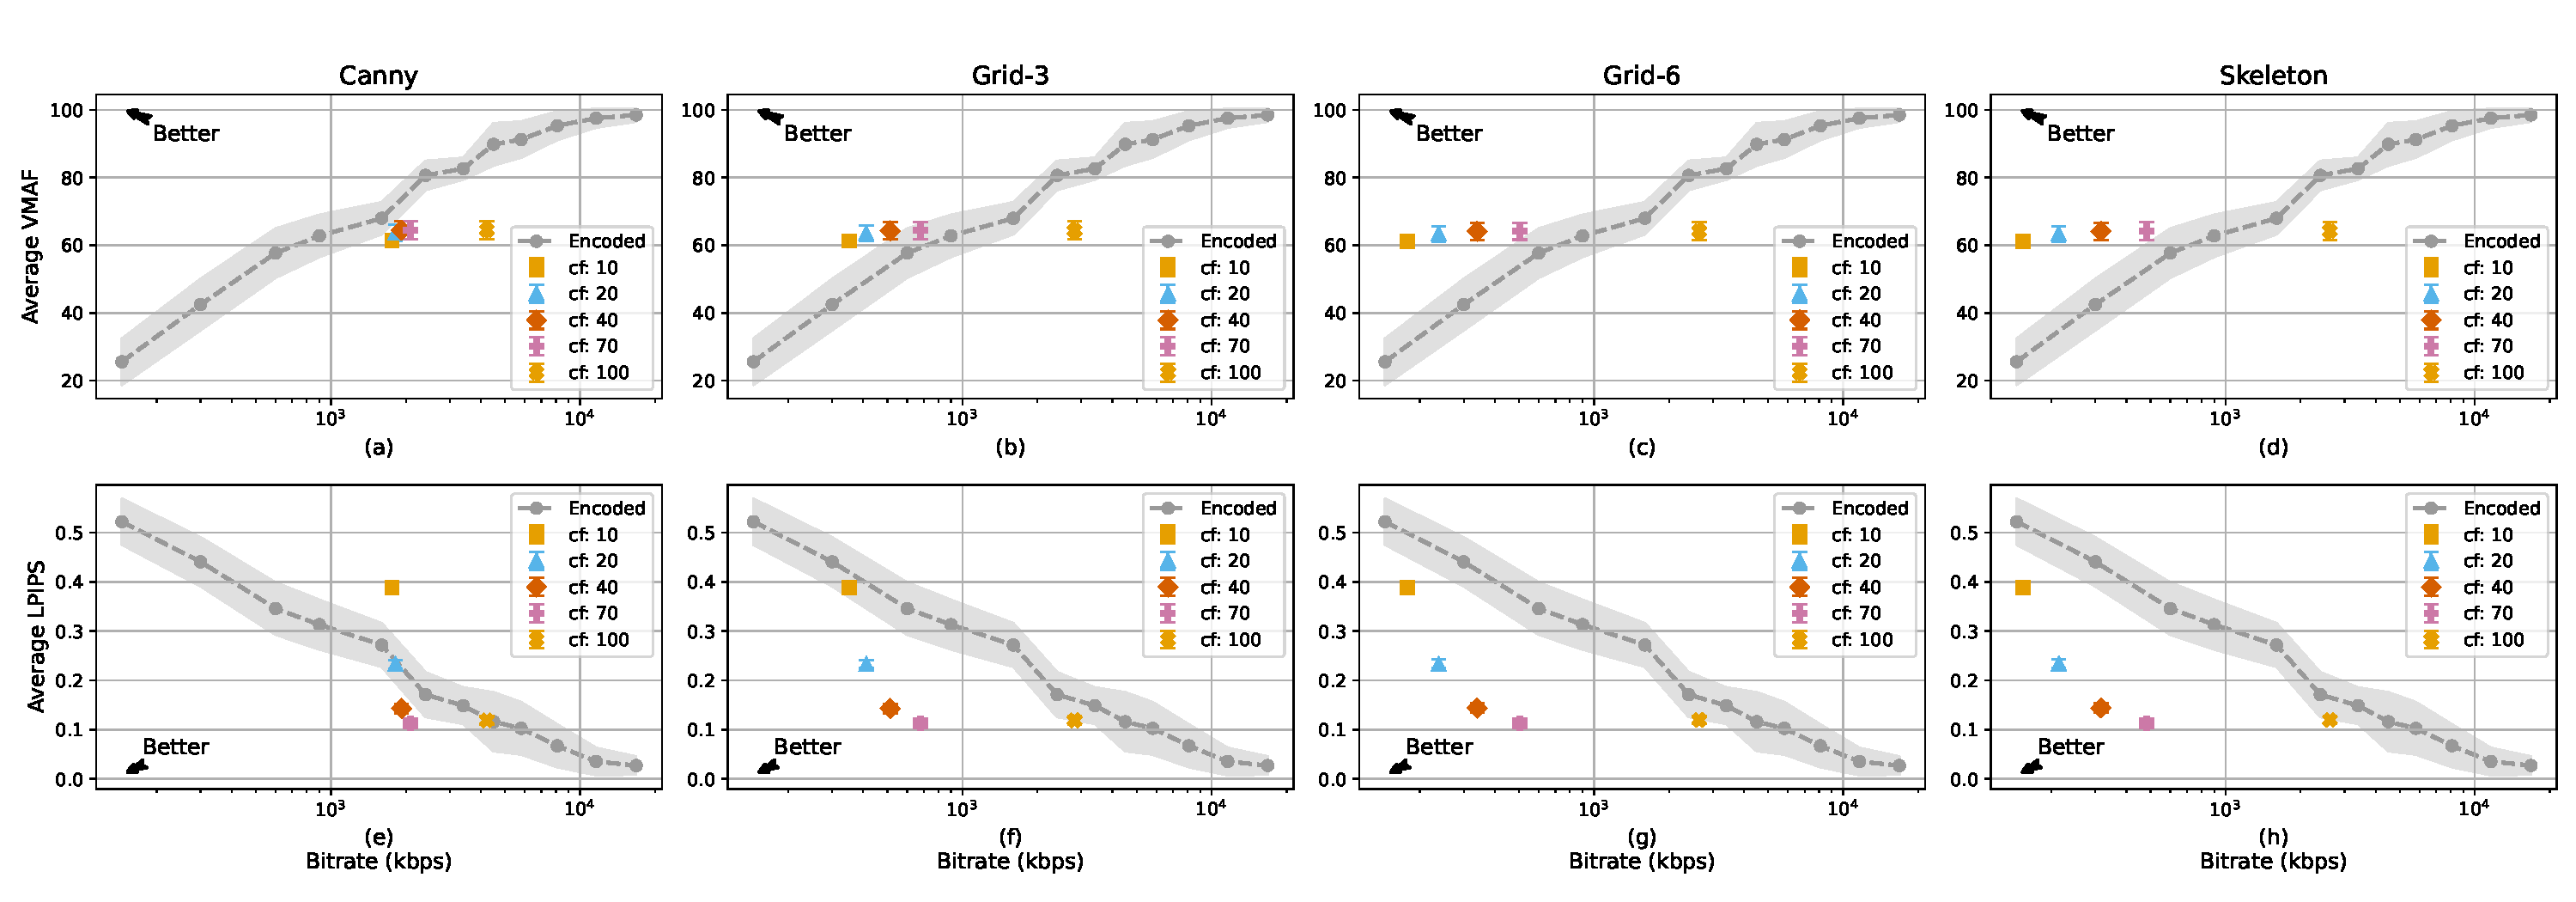
\includegraphics[width=1\linewidth]{figures/vmaf-lpips_vs_bitrate_dualrow.pdf}
    \caption{Average VMAF and LPIPS across all frames for different generation methods, background compression factors (cf), and encoded representations across segment lengths (with 95\% confidence interval in gray).}
    \label{fig:vmaf-lpips-bitrate}
\end{figure*}
\subsubsection*{Model size and scalability}
The final scenario investigates the effect of model size on reconstruction quality. We evaluate models trained on the same data, Scene 24, at varying resolutions, from \vxv{128}{128} to \vxv{1024}{1024}. Note that no data from Scene 24 was used during the training phase. This comparison highlights how increasing model complexity impacts performance. It is important to highlight that we utilized DeepCABAC~\cite{wiedemann2019deepcabac} to compress the network weights by \qty{69}{\percent} with negligible quality loss, resulting in the outcomes shown in Table~\ref{tab:scenario2}. This step is critical for minimizing the amount of data transmitted to the client. Since these models are player-specific and not match-specific, they can be trained in advance and delivered to the client before the streaming session begins—such as during idle periods in the days preceding a match concerning a particular player. This avoids incurring any real-time bandwidth cost and ensures that the client is equipped to decode the transmitted keypoint data efficiently throughout the session.
However, a practical deployment of PointStream would greatly benefit from a more general model capable of synthesizing arbitrary players. Such a model is in active development and is left as a promising direction for future work.

As shown in Table~\ref{tab:scenario2}, increasing the size of the generative models does not yield significant improvements in quality metrics. Instead, overall visual quality is much more tied to the quality of the background. This is likely due to two factors: players occupy a relatively small portion of the frame, and the task of reconstructing a specific player is relatively easy when provided with detailed pose or spatial information.
Given that our models already achieve inference speeds on average above \num{57}\,fps and can be delivered to the client ahead of time, we consider further optimization of model architecture or size to be outside the scope of this work.


% Furthermore, we analyzed the bitrates of the distorted video files to assess PointStream’s compression efficiency compared to HEVC, examining the trade-off between file size and perceptual quality. Lastly, we evaluate the total execution time, \ie the time required to process a video through PointStream’s entire pipeline -- from video capture to scene reconstruction. We then compared it against HEVC’s encoding time to evaluate the feasibility of PointStream for real-time applications and potential use cases in live streaming. % Maybe only the feasibility for real-time applications

% \subsection{Results and analysis}\label{subsec:results}
% % \subsubsection{Quantitative and qualitative comparisons}
% We conduct a comprehensive comparison between our PointStream and
% several state-of-the-art X methods, including X, Y, Z.


% \noindent

% \textbf{Quantitative comparison.} Table with results about PSNR etc.

% \noindent

% \textbf{Qualitative comparison.} Exemplar visual results for various methods are presented in Figure X. PointStream generates high-quality...

% \noindent
% \textbf{Dataset.}

% \noindent

% \noindent
% \textbf{Evaluation metrics.}

% \noindent
% \textbf{Implementation details.}



% \subsection{Ablation study}

% Ablation study here.

\section{Conclusion}
In this paper, we introduced PointStream, a new approach to live video streaming that leverages semantic compression and generative reconstruction to transmit human-centric video content with unprecedented efficiency. PointStream encodes only the essential semantic information -- such as object keypoints -- and reconstructs high-fidelity video on the client side through learned generative models.
We then showed how an implementation of PointStream tailored to tennis matches achieves the same video quality as traditional live encoders at up to \num{10} times less bitrate, thanks to a modular end-to-end pipeline that integrates SOTA pose estimation, segmentation, and background modeling into a practical streaming solution.
Despite these achievements, the current implementation is still quite specialized. While the system architecture can apply to any tennis match, generalize to other sports with minimal modification, and potentially to broader video categories with further adaptation, highly varied content (\eg movies) remains a challenge. A practical deployment would likely adopt a hybrid strategy -- applying PointStream to predictable, human-centric scenes and falling back to traditional codecs for others.

Furthermore, a significant open challenge lies in evaluating perceptual quality for AI-generated reconstructions. While VMAF and LPIPS offer a good approximation, they may not fully capture perceptual realism in generated videos. Future work includes developing tailored quality metrics and conducting subjective user studies to validate viewer experience and comfort.
% From a deployment perspective, PointStream requires careful consideration. Its reliance on compute-intensive generative models suggests a need for edge compute scenarios, such as live sports streaming powered by on-site edge servers.

Overall, PointStream represents a shift toward cognitive-inspired streaming -- prioritizing what the viewer needs to perceive rather than faithfully transmitting every pixel. We believe this paradigm has the potential to reshape how we think about video compression, particularly in domains where human understanding and photorealistic fidelity can be decoupled from raw data volume.

%\newpage

%\section{Acknowledgments}
%The financial support of the Austrian Federal Ministry for Digital and Economic Affairs, the National Foundation for Research, Technology and Development, and the Christian Doppler Research Association, is gratefully acknowledged. Christian Doppler Laboratory ATHENA: https://athena.itec.aau.at/

%%
%% The next two lines define the bibliography style to be used, and
%% the bibliography file.
\bibliographystyle{ACM-Reference-Format}
\bibliography{ref}

%%
%% If your work has an appendix, this is the place to put it.
%\appendix

%\section{Section I}

%\subsection{Subsection I}

%Lorem ipsum dolor sit amet, consectetur adipiscing elit.

\end{document}
\endinput
%%
%% End of file `sample-sigconf.tex'.
